\documentclass[a4paper,12pt]{article}
\usepackage{amssymb}
\usepackage{amsfonts}
\usepackage{amsthm}
\usepackage{amsmath}
\usepackage[T1]{fontenc}
\usepackage[utf8]{inputenc}
\usepackage[british]{babel}
\usepackage{times}
\usepackage{anysize}
\usepackage{color}
\usepackage{listings}
\usepackage{graphicx}
\usepackage{enumerate}
\usepackage{multicol}
\usepackage{float}

\usepackage{lmodern}  % for bold teletype font
\usepackage{xcolor}   % for \textcolor
%\lstloadlanguages{matlab}
\lstset{
	basicstyle=\ttfamily,
	columns=fullflexible,
%	frame=single,
	breaklines=true,
	postbreak=\mbox{\textcolor{red}{$\hookrightarrow$}\space},
}

\begin{document}
\begin{titlepage}
\center
\vspace*{\fill}
\Huge{Modeling of Physical Systems}\\
\Large{Taylor model, explicit method}\\
\vspace*{1.5cm}
Dominik Katszer\\
\large{28 April 2018}
\vspace*{1.5cm}
\vspace*{\fill}
\end{titlepage}
\section{Aim of laboratory}

The aim of the laboratory is to create a simple numerical model simulating one dimensional
transport of the pollutants in the river using QUICKEST explicit method. During simulation mass conservation law have to be preserved, which should be shown in the plot. 
Transport of pollutants should be measured in 90m of the river and presented in a time-depentent plot.
\section{Algorithm}
Simulation was performed using explicit method which allows to calculate the function value in $n+1$ time step based on values assigned to $n$ time step only.
\\
\centerline{
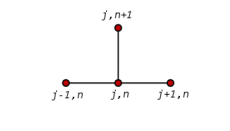
\includegraphics[scale=1]{explicitMethod.png}
}
Spatial and temporal distribution of conservative tracer in the river was calculated using iteration formula named Quickest method. Details of this algorithm are presented below.
\\
\centerline{
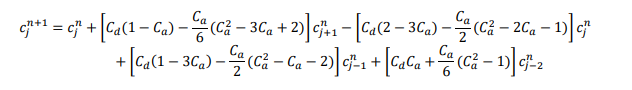
\includegraphics[scale=1]{quickestEq.png}
}
where:
\begin{description}
\item $C_a = \frac{U\Delta t}{\Delta x}$ – advective Courant number
\item $C_d = \frac{D\Delta t}{\Delta x^2}$ - diffusive Courant number
\end{description}
What is more boundary conditions which are enumerated below had to be preserved. 
\begin{itemize}
\item left-side -- Dirichlet condition
$$
c(0,t) = 0
$$
\item right-side -- von Neumann condition
$$
\frac{\partial c}{\partial x}(L,t) = 0
$$
\end{itemize}

Additional initial condition:
\\
\centerline{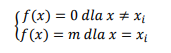
\includegraphics[scale=1]{initialCond.png}}
where :
\begin{description}
\item $m$ -- initial concentration in the injection point
\item $x_i$ --  location of the injection point
\end{description}
\subsection{Input Data}
\begin{itemize}
\item \verb!riverLength = 100! -- length of the river $[m]$ 
\item \verb!riverWidth = 5! -- width of the river $[m]$
\item \verb!riverDepth = 1! -- depth of the river $[m]$
\item \verb!U = 0.1! -- mean flow velocity $[m/s]$
\item \verb!D = 0.01! -- dispersion coefficient $[m/s^2]$
\item location of the injection point $10m$
\item location of the measurement point $90m$
\item \verb!wieghtOfTracer = 1! -- amount of injected tracer $[kg]$
\end{itemize}
\section{Results}
\subsection{Tracer concentration}
\centerline{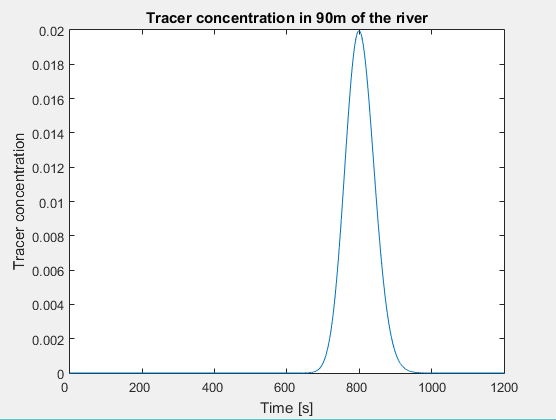
\includegraphics[scale=1]{tracerConcetration}}
Because of water flow, the injected tracer approached 90m in the around 800 seconds. Tracer is spreading in the river that why we can observe that around 725 and 875 second there is not such intensive concentration as in 800s.
\subsection{Totall mass of tracer in the river}
\centerline{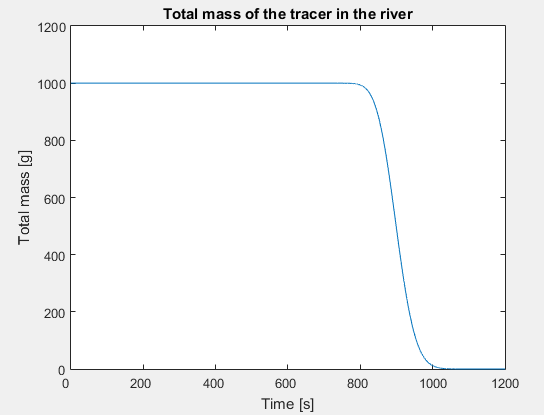
\includegraphics[scale=1]{totalMass}}
We can observe that totall mass of tracer is always the same in the river till the end where tracer leaves the part of river under simulation.
\section{Conclusions}
This laboratory shows how to simplify model. River is three dimensional but we did not need such amount of information so we could use only one dimension. What is more I achieved all aims and all plots describes very well the flow of the tracer in the river.
\section{Source code}
\lstinputlisting{taylorModel.m}

\end{document}